\documentclass[12pt]{article}
\usepackage[T2A]{fontenc}
\usepackage[utf8]{inputenc}
\usepackage{multirow}
\usepackage{caption}
\usepackage{subcaption}
\usepackage{amsmath}
\usepackage{changepage}
\usepackage{graphicx}
\usepackage{float}
\usepackage[english,russian]{babel}
\usepackage{amsmath, amsfonts, amssymb, amsthm, mathtools}
\usepackage{xcolor}
\usepackage{array}
\usepackage{hyperref}
\usepackage[top = 1.5cm, left = 1.5 cm, right = 1.5 cm, bottom = 3 cm]{geometry}
\graphicspath{ {./images/} }
 
\title{Определение моментов диссипативных сил гироскопа}
\author{Шахматов Андрей, Б02-304}
\date{\today}
  
\begin{document}
\begin{titlepage}
    \begin{center}
        {\large МОСКОВСКИЙ ФИЗИКО-ТЕХНИЧЕСКИЙ ИНСТИТУТ (НАЦИОНАЛЬНЫЙ ИССЛЕДОВАТЕЛЬСКИЙ УНИВЕРСИТЕТ)}
    \end{center}
    \begin{center}
        {\large Физтех-школа физики и исследований им. Ландау}
    \end{center}
    
    
    \vspace{3cm}
    {\huge
        \begin{center}
            \textbf{Определение модуля Юнга с помощью деформации изгиба}
        \end{center}
    }
    \vspace{2cm}
    \begin{flushright}
        {\LARGE Автор:\\ Шахматов Андрей Юрьевич \\
            \vspace{0.2cm}
            Б02-304}
    \end{flushright}
    \vspace{7 cm}
    \begin{center}
        Долгопрудный 2023
    \end{center}
\end{titlepage}

% \maketitle

\begin{abstract}
    Исследованы прогибы нескольких балок в зависимости от подвешиваемой нагрузки для различных материалов. Найдены геометрические параметры балок.
    Определены модули Юнга каждой из балок. Полученные результаты сравнены с табличными значениями модулей Юнга для материалов балок.
\end{abstract}

\tableofcontents

\section{Введение}
Важной задачей материаловедения и строительной инженерии является определение механических свойств материалов, 
одним из которых является модуль Юнга. Классический метод определения модуля Юнга заключается в приложении механического напряжения $\sigma$
к трубке из исследуемого материала и измерении относительного удлинения $\epsilon$ этой трубки. Модуль Юнга может быть найден как отношение 
механического напряжения к удлинению: $E = \frac{\sigma}{\epsilon}$. Однако этот метод неэффективен для определения модуля Юнга в твёрдых телах, 
так как требует огромного напряжения для достижения достаточного удлинения. Хотя существуют и другие методы измерения модуля Юнга, 
одним из них является измерение прогиба балки из исследуемого материала и вычисление модуля Юнга на основе зависимости прогиба от нагрузки. 
Этот метод не имеет недостатков предыдущего метода, поскольку для измерения даже достаточно твёрдых материалов можно использовать нагрузку массой, 
не превышающей килограмм. Цель текущей работы заключается в исследовании прогиба нескольких балок из различных материалов и определении их 
модулей Юнга.

\section{Методика}
В эксперименте была использована установка, изображённая на рисунке \ref{fig:1}.
\begin{figure}
    \begin{center}
        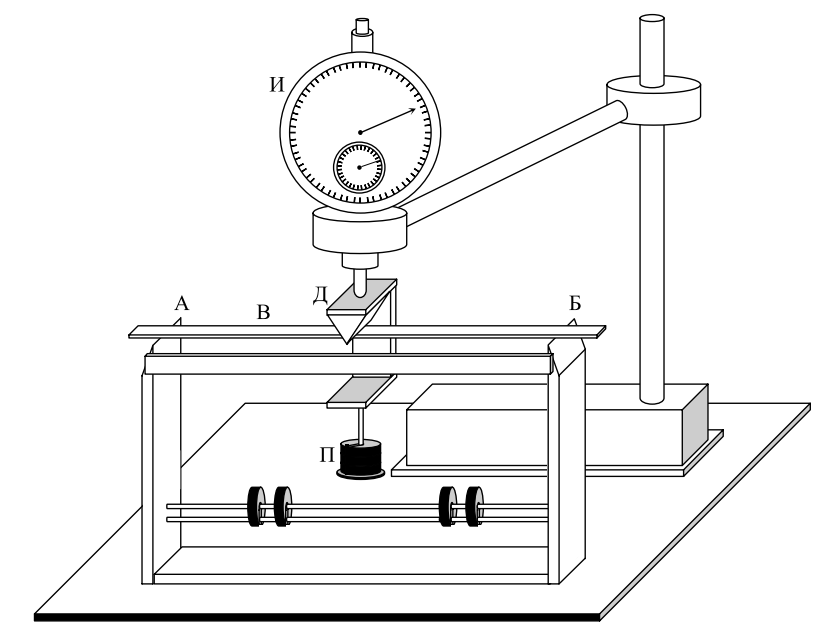
\includegraphics[width=0.7\textwidth]{im.png}
    \end{center}
    \caption{Экспериментальная установка, состоящая из прочной стойки с опорными призмами А и Б.
        На рёбра призм опирается исследуемый объект В. В середине стержня на призме Д подвешена площадка П с грузами. 
        Измерять стрелу прогиба можно с помощью индикатора И, укрепляемого на отдельной штанге. 
        Полный оборот большой стрелки индикатора соответствует 1 мм и одному делению малого циферблата.}
    \label{fig:1}
\end{figure}
Согласно \cite{LabBook}, в случае небольших прошибов балки, возможно связать максимальный прогиб $y_{max}$ с толщиной балки $b$, длиной балки $l$,
шириной балки $a$, силой, приложенной к балке, $P$ и модулем Юнга балки $E$ выражением
\begin{equation}\label{eq:1}
    y_{max} = \frac{Pl^3}{4ab^3E}
\end{equation}
Тогда введя для каждой балки геометрический коэффициент $k = \frac{4ab^3}{l^3}$ и определив коэффициент наклона графика 
$y_{max}(P)$ $q$, можно найти модуль Юнга балки $E = \frac{1}{kq}$.

\section{Результаты и их анализ}
При помощи штангенциркуля были измерены размеры трех балок: их ширина $a$ и толщина $b$ в 10 точках в целях уменьшения случайной погрешности измерений, 
результаты были усреднены по 10 измерениям (Таблица \ref{tab:1}). Для каждой из 3 балок были измерены зависимости прогиба балки от приложенной
нагрузки (Таблица \ref{tab:2}), измерения проводились как на увеличение подвешиваемой нагрузки, так и на уменьшение. 
Также измерены зависимости прогиба от нагрузки для перевернутой балки (Таблица \ref{tab:3}) и для балки, 
точка приложения нагрузки которой смещена на 1 \% длины от центра балки (Таблица \ref{tab:4}). Для каждой из балок построены графики зависимости прогиба в 
случае увеличения нагрузки и в случае уменьшения нагрузки (Рис. \ref{fig:2}, \ref{fig:3}, \ref{fig:4}). 
Из графиков сделан вывод о том, что зависимость прогиба балки не зависит от того, увеличивается масса нагрузки или уменьшается. 
Из графика (Рис \ref{fig:5}) прогиба балки при смещённой точке подвеса грузов следует, что небольшое смещение от центра подвеса не влияет на зависимость.
Для каждой из перевёрнутых балок построены графики зависимости прогиба от нагрузки (Рис. \ref{fig:5}, \ref{fig:6}, \ref{fig:7}). Из графиков сделан
вывод о наличие пластической деформации у исследуемых материалов, потому в дальнейших расчётах модуля Юнга будут использоваться данные, полученные
на неперевёрнутых балках.
Построен общий график зависимости прогиба для 3 балок (Рис. \ref{fig:9}).
\begin{figure}[H]
    \begin{center}
        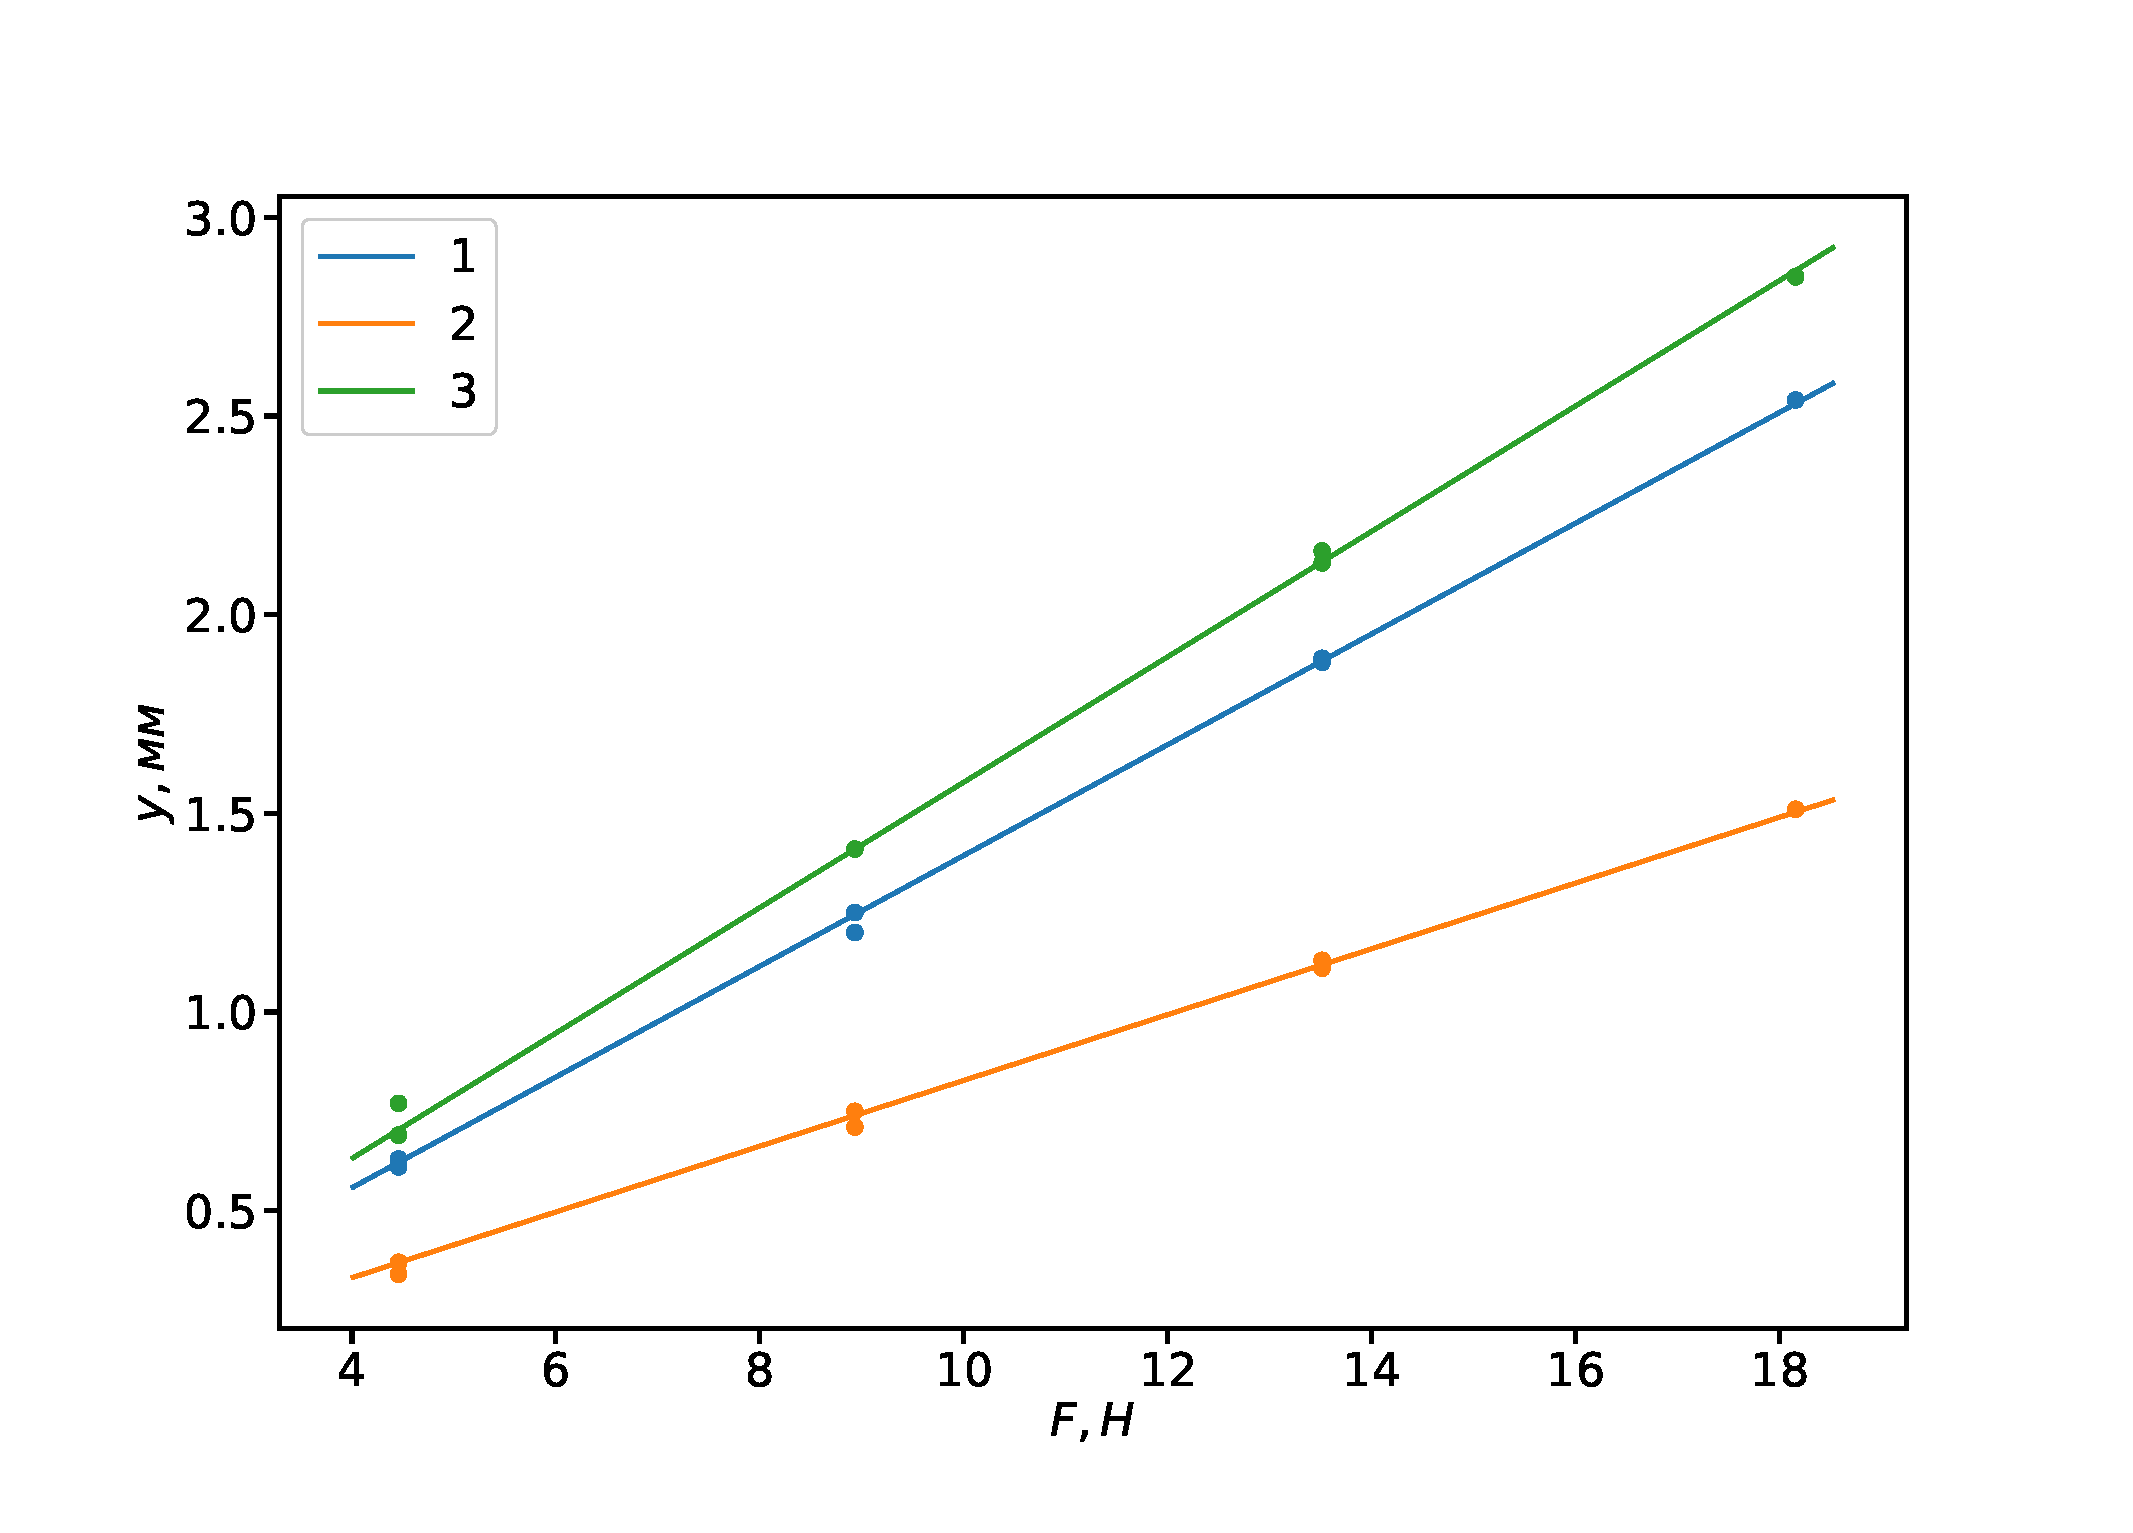
\includegraphics[width=0.8\textwidth]{gr123.eps}
    \end{center}
    \caption{Сгруппированный график зависимости прогиба балки от нагрузки, приложенной к центру балки. Материалы балок: 1 - железная балка, 
    2 - дубовая балка, 3 - еловая балка.}
    \label{fig:9}
\end{figure}
Коэффициенты наклона соответствующие цифрам на графике \ref{fig:9} равны $k_1 = (1.394 \pm 0.006) \cdot 10^{-4}$ $\frac{\textrm{м}}{\textrm{Н}}$, 
$k_2 = (8.28 \pm 0.05) \cdot 10^{-5}$ $\frac{\textrm{м}}{\textrm{Н}}$, $k_3 = (1.578 \pm 0.008) \cdot 10^{-4}$ $\frac{\textrm{м}}{\textrm{Н}}$.
Тогда модули соответствующие модули Юнга равны $E_1 = (2.01 \pm 0.19) \cdot 10^{11} \textrm{ Па}$, 
$E_2 = (1.68 \pm 0.13) \cdot 10^{10} \textrm{ Па}$, $E_3 = (1.01 \pm 0.06) \cdot 10^{10} \textrm{ Па}$. Полученные модули Юнга соответствуют табличным
значениям модулей Юнга для железа $E_{t_1} = 2.00 \cdot 10^{11} \textrm{ Па}$, дуба $E_{t_2} = 1.54 \cdot 10^{10} \textrm{ Па}$ и 
ели $E_{t_3} = 1.10 \cdot 10^{10} \textrm{ Па}$, согласно \cite{ValuesBook}.

\section{Выводы}
Пластические деформации балок оказались меньше $0.01$ мм, тогда как минимальная упругая деформация оказалась равна $0.5$ мм.
Так как пластическая деформация окалась в $50$ раз меньше упругой можно считать модель упругих деформаций корректной для поставленной задачи.
Измеренные модули Юнга составили $E_1 = (2.01 \pm 0.19) \cdot 10^{11} \textrm{ Па}$, 
$E_2 = (1.68 \pm 0.13) \cdot 10^{10} \textrm{ Па}$, $E_3 = (1.01 \pm 0.06) \cdot 10^{10} \textrm{ Па}$. Полученные значения совпали с табличными
значениями для железа, дуба и ели в пределах погрешности.

\section{Использованная литература}
\begin{thebibliography}{9}
    \bibitem{LabBook}
    Лабораторный практикум по общей физике, Том 1, под редакцией А. Д. Гладуна
    \bibitem{ValuesBook}
    Таблицы физических величин. Справочник / Под ред. И.К. Кикоина. М., Атомиздат. 1976, 1008 с.
\end{thebibliography}

\section{Приложения}
\subsection{Геометрические характеристики балок} \label{app_1}
\begin{table}[H]
    \centering
    \begin{tabular}{|r|r|r|r|r|r|}
        \hline
        \multicolumn{2}{|c|}{Железная балка} & 
        \multicolumn{2}{|c|}{Дубовая балка}  & 
        \multicolumn{2}{|c|}{Еловая балка}                                                     \\
        \hline
        $a$, см                              & $b$, см & $a$, см & $b$, см & $a$, см & $b$, см \\
        \hline
        2.12                                 & 0.39    & 1.86    & 1.07    & 2.06    & 1.03    \\
        2.10                                 & 0.39    & 1.84    & 1.05    & 2.02    & 1.01    \\
        2.07                                 & 0.38    & 1.84    & 1.05    & 1.99    & 1.00    \\
        2.09                                 & 0.38    & 1.84    & 1.05    & 1.98    & 1.01    \\
        2.12                                 & 0.38    & 1.83    & 1.09    & 2.00    & 0.99    \\
        2.13                                 & 0.38    & 1.83    & 1.10    & 2.03    & 1.00    \\
        2.15                                 & 0.39    & 1.90    & 1.11    & 2.01    & 0.99    \\
        2.14                                 & 0.37    & 1.93    & 1.12    & 2.03    & 1.01    \\
        2.11                                 & 0.38    & 1.83    & 1.09    & 2.00    & 1.01    \\
        2.12                                 & 0.38    & 1.90    & 1.11    & 2.06    & 1.02    \\
        \hline
    \end{tabular}
    
    \caption{Геометрические размеры балок. $a$ - ширина балки, $b$ - толщина балки}
    \label{tab:1}
\end{table}
Для каждой из трёх балок рассчитан геометрический коэффициент $k = \frac{4ab^3}{l^3}$: $k_1 = (3.6 \pm 0.4) \cdot 10^{-8}$ м, $k_2 = (7.2 \pm 0.6) \cdot 10^{-7}$ м,
$k_1 = (6.3 \pm 0.4) \cdot 10^{-7}$ м.
\subsection{Данные исследования прогиба балки от приложенной нагрузки в различных условиях} \label{app_2}
\begin{table}[H]
    \centering
    \begin{tabular}{|r|r|r|r|r|r|r|}
        \hline
        \multicolumn{3}{|c|}{Железная балка} & 
        \multicolumn{2}{|c|}{Дубовая балка}  & 
        \multicolumn{2}{|c|}{Еловая балка}                                                            \\
        \hline
                                             & $m$, г & $y$, мм & $m$, г & $y$, мм & $m$, г & $y$, мм \\
        \hline
        0                                    & 454.8  & 0.61    & 454.8  & 0.34    & 454.8  & 0.69    \\
        1                                    & 911.4  & 1.25    & 911.4  & 0.71    & 911.4  & 1.41    \\
        2                                    & 1379.0 & 1.88    & 1379.0 & 1.11    & 1379.0 & 2.13    \\
        3                                    & 1852.9 & 2.54    & 1852.9 & 1.51    & 1852.9 & 2.85    \\
        4                                    & 1852.9 & 2.54    & 1852.9 & 1.51    & 1852.9 & 2.85    \\
        5                                    & 1379.0 & 1.89    & 1379.0 & 1.13    & 1379.0 & 2.16    \\
        6                                    & 911.4  & 1.20    & 911.4  & 0.75    & 911.4  & 1.41    \\
        7                                    & 454.8  & 0.63    & 454.8  & 0.37    & 454.8  & 0.77    \\
        \hline
    \end{tabular}
    
    \caption{Данные измерения прогиба балок от приложенного механического напряжения к её центру. $y$ - максимальный прогиб балки,
        $m$ - масса нагрузки. Измерения, номер которых меньше 4 проводились при увеличении нагрузки, приложенной к балке, измерения с номером больше 3 проводились при уменьшении приложенной нагрузки}
    \label{tab:2}
\end{table}

\begin{table}[H]
    \centering
    \begin{tabular}{|r|r|r|r|r|r|r|}
        \hline
        \multicolumn{3}{|c|}{Железная балка} & 
        \multicolumn{2}{|c|}{Дубовая балка}  & 
        \multicolumn{2}{|c|}{Еловая балка}                                                            \\
        \hline
                                             & $m$, г & $y$, мм & $m$, г & $y$, мм & $m$, г & $y$, мм \\
        \hline
        0                                    & 454.8  & 0.64    & 454.8  & 0.37    & 454.8  & 0.76    \\
        1                                    & 911.4  & 1.25    & 911.4  & 0.75    & 911.4  & 1.39    \\
        2                                    & 1379.0 & 1.91    & 1379.0 & 1.16    & 1379.0 & 2.11    \\
        3                                    & 1852.9 & 2.61    & 1852.9 & 1.56    & 1852.9 & 2.84    \\
        4                                    & 1852.9 & 2.61    & 1852.9 & 1.56    & 1852.9 & 2.84    \\
        5                                    & 1379.0 & 1.95    & 1379.0 & 1.17    & 1379.0 & 2.15    \\
        6                                    & 911.4  & 1.33    & 911.4  & 0.78    & 911.4  & 1.45    \\
        7                                    & 454.8  & 0.72    & 454.8  & 0.38    & 454.8  & 0.77    \\
        \hline
    \end{tabular}
    
    \caption{Данные измерения прогиба перевёрнутых балок от приложенного механического напряжения к её центру. $y$ - максимальный прогиб балки,
        $m$ - масса нагрузки. Измерения, номер которых меньше 4 проводились при увеличении нагрузки, приложенной к балке, измерения с номером больше 3 проводились при уменьшении приложенной нагрузки}
    \label{tab:3}
\end{table}

\begin{table}[H]
    \centering
    \begin{tabular}{|r|r|r|}
        \hline
        \multicolumn{3}{|c|}{Железная балка} \\
        \hline
          & $m$, г & $y$, мм                 \\
        \hline
        0 & 454.8  & 0.59                    \\
        1 & 911.4  & 1.22                    \\
        2 & 1379.0 & 1.88                    \\
        3 & 1852.9 & 2.54                    \\
        4 & 1852.9 & 2.54                    \\
        5 & 1379.0 & 1.89                    \\
        6 & 911.4  & 1.26                    \\
        7 & 454.8  & 0.64                    \\
        \hline
    \end{tabular}
    
    \caption{Данные измерения прогиба балки от приложенного механического напряжения к её точке, удалённой от центра на несколько милиметров. $y$ - максимальный прогиб балки,
        $m$ - масса нагрузки. Измерения, номер которых меньше 4 проводились при увеличении нагрузки, приложенной к балке, измерения с номером больше 3 проводились при уменьшении приложенной нагрузки}
    \label{tab:4}
\end{table}

\subsection{Графики, построенные на данных из таблиц из приложения \ref{app_2}} \label{app_3}
\begin{figure}[H]
    \begin{center}
        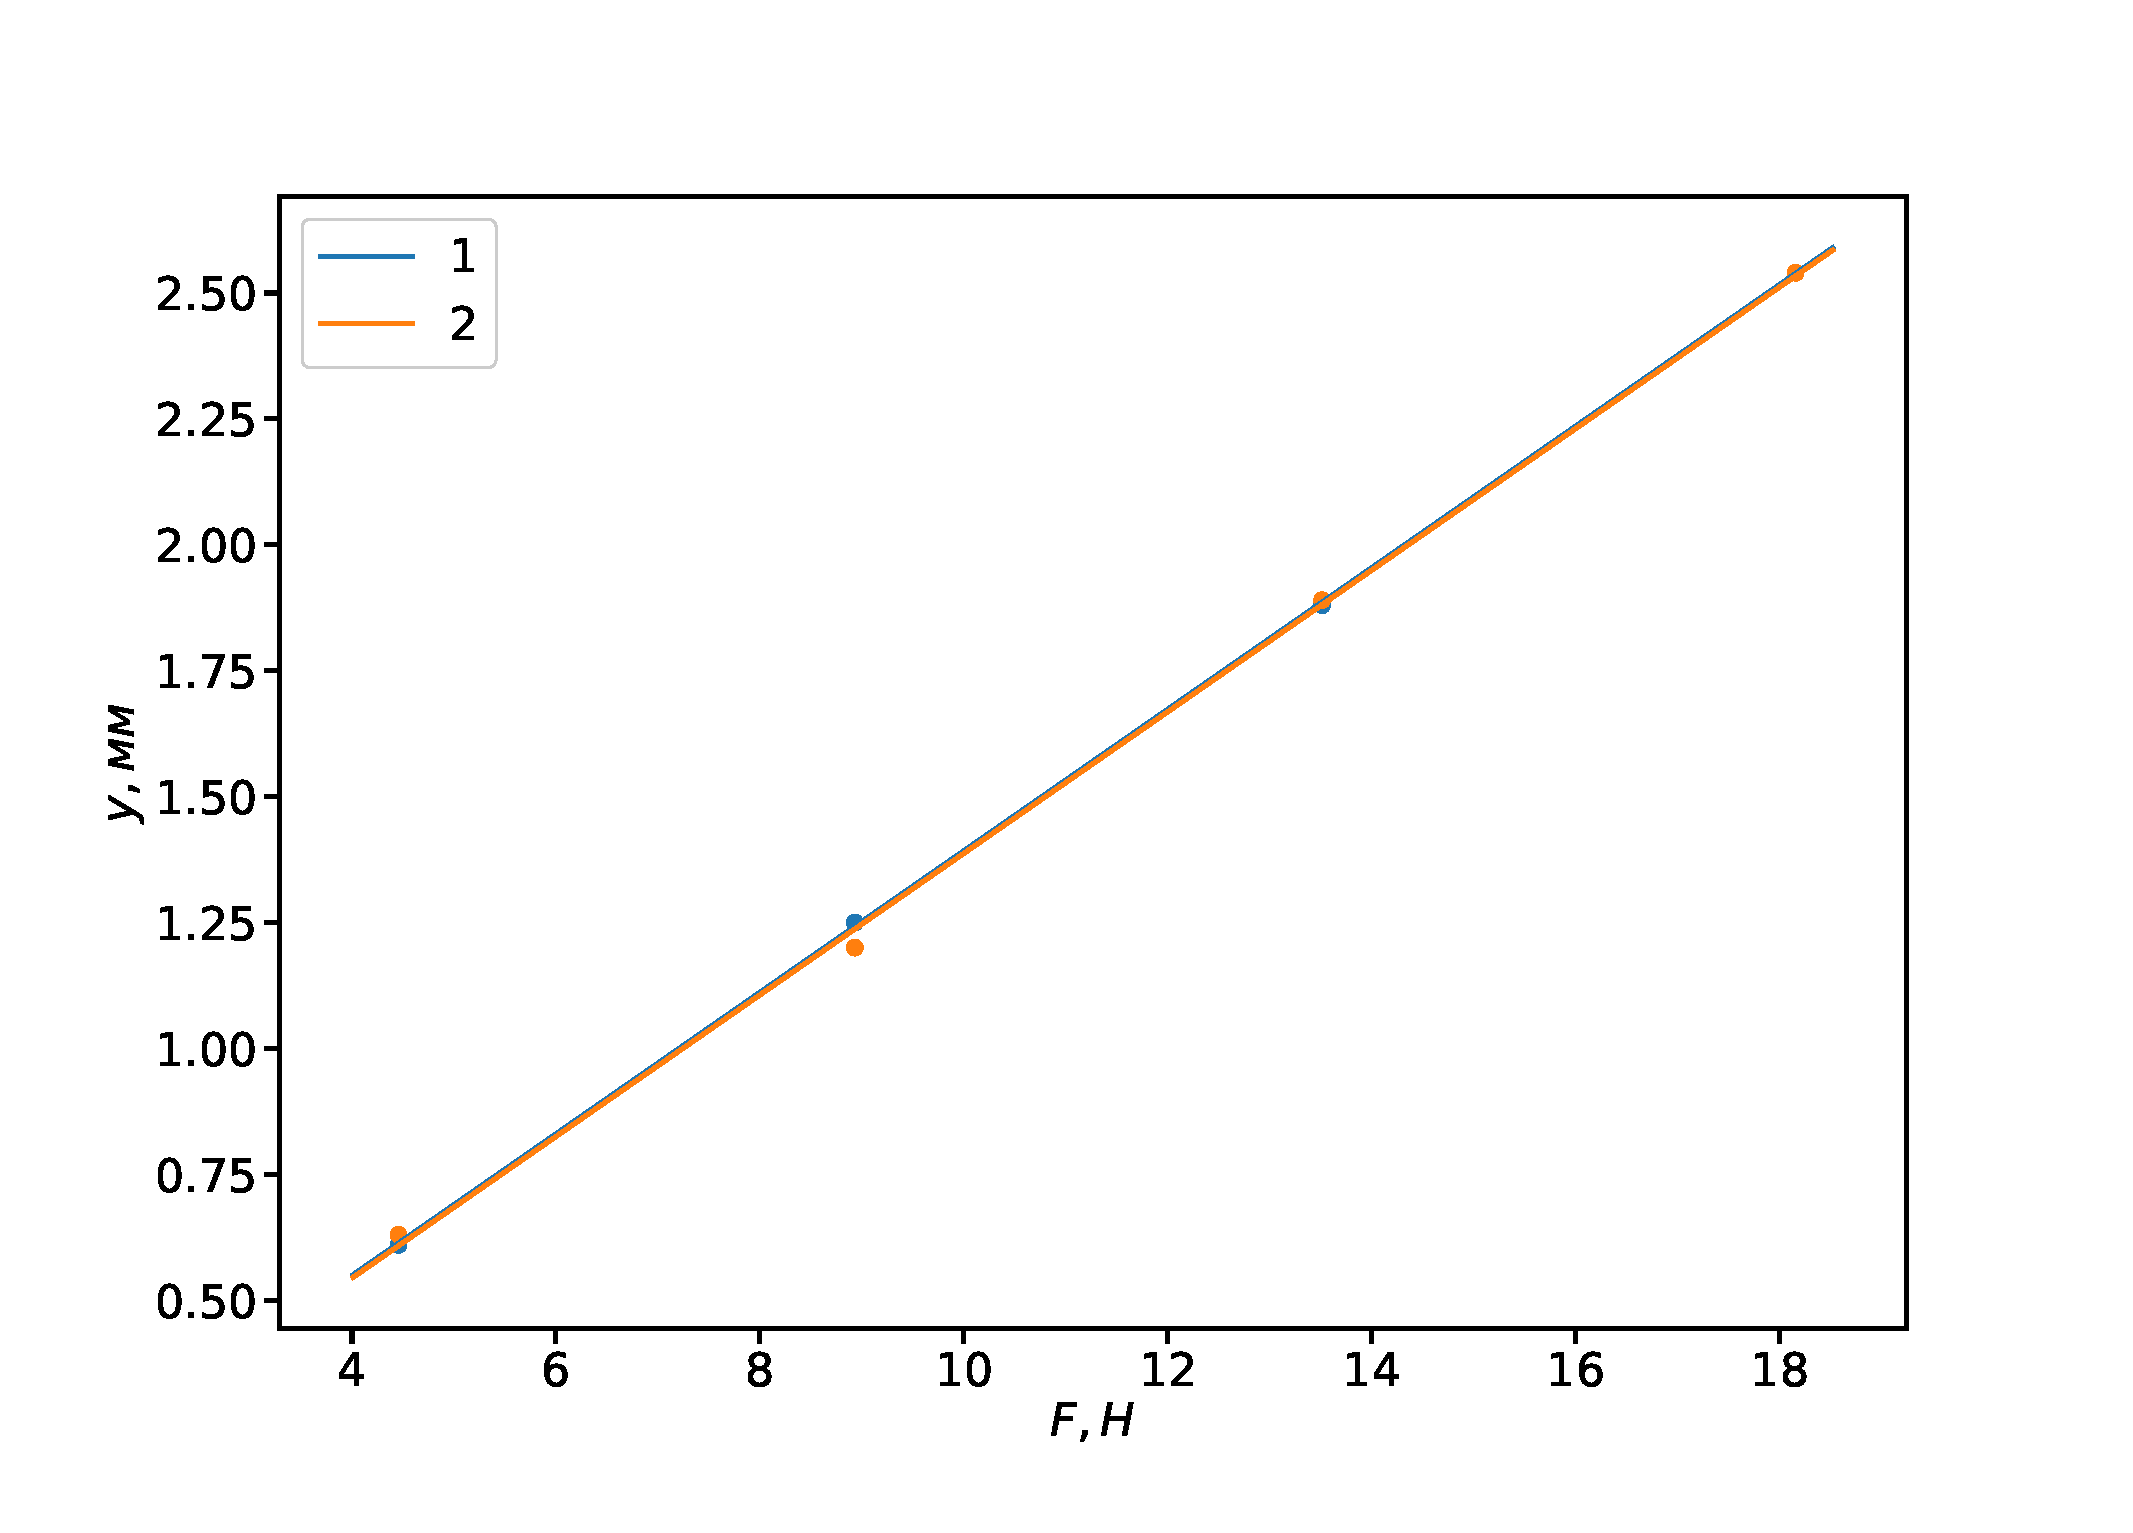
\includegraphics[width=0.6\textwidth]{groupdown_metal.eps}
    \end{center}
    \caption{Графики зависимости максимального прогиба железной балки $y$ от приложенной нагрузки $F$. 1 - измерение на увеличение нагрузки.
        2 - измерение на уменьшение нагрузки.}
    \label{fig:2}
\end{figure}

\begin{figure}[H]
    \begin{center}
        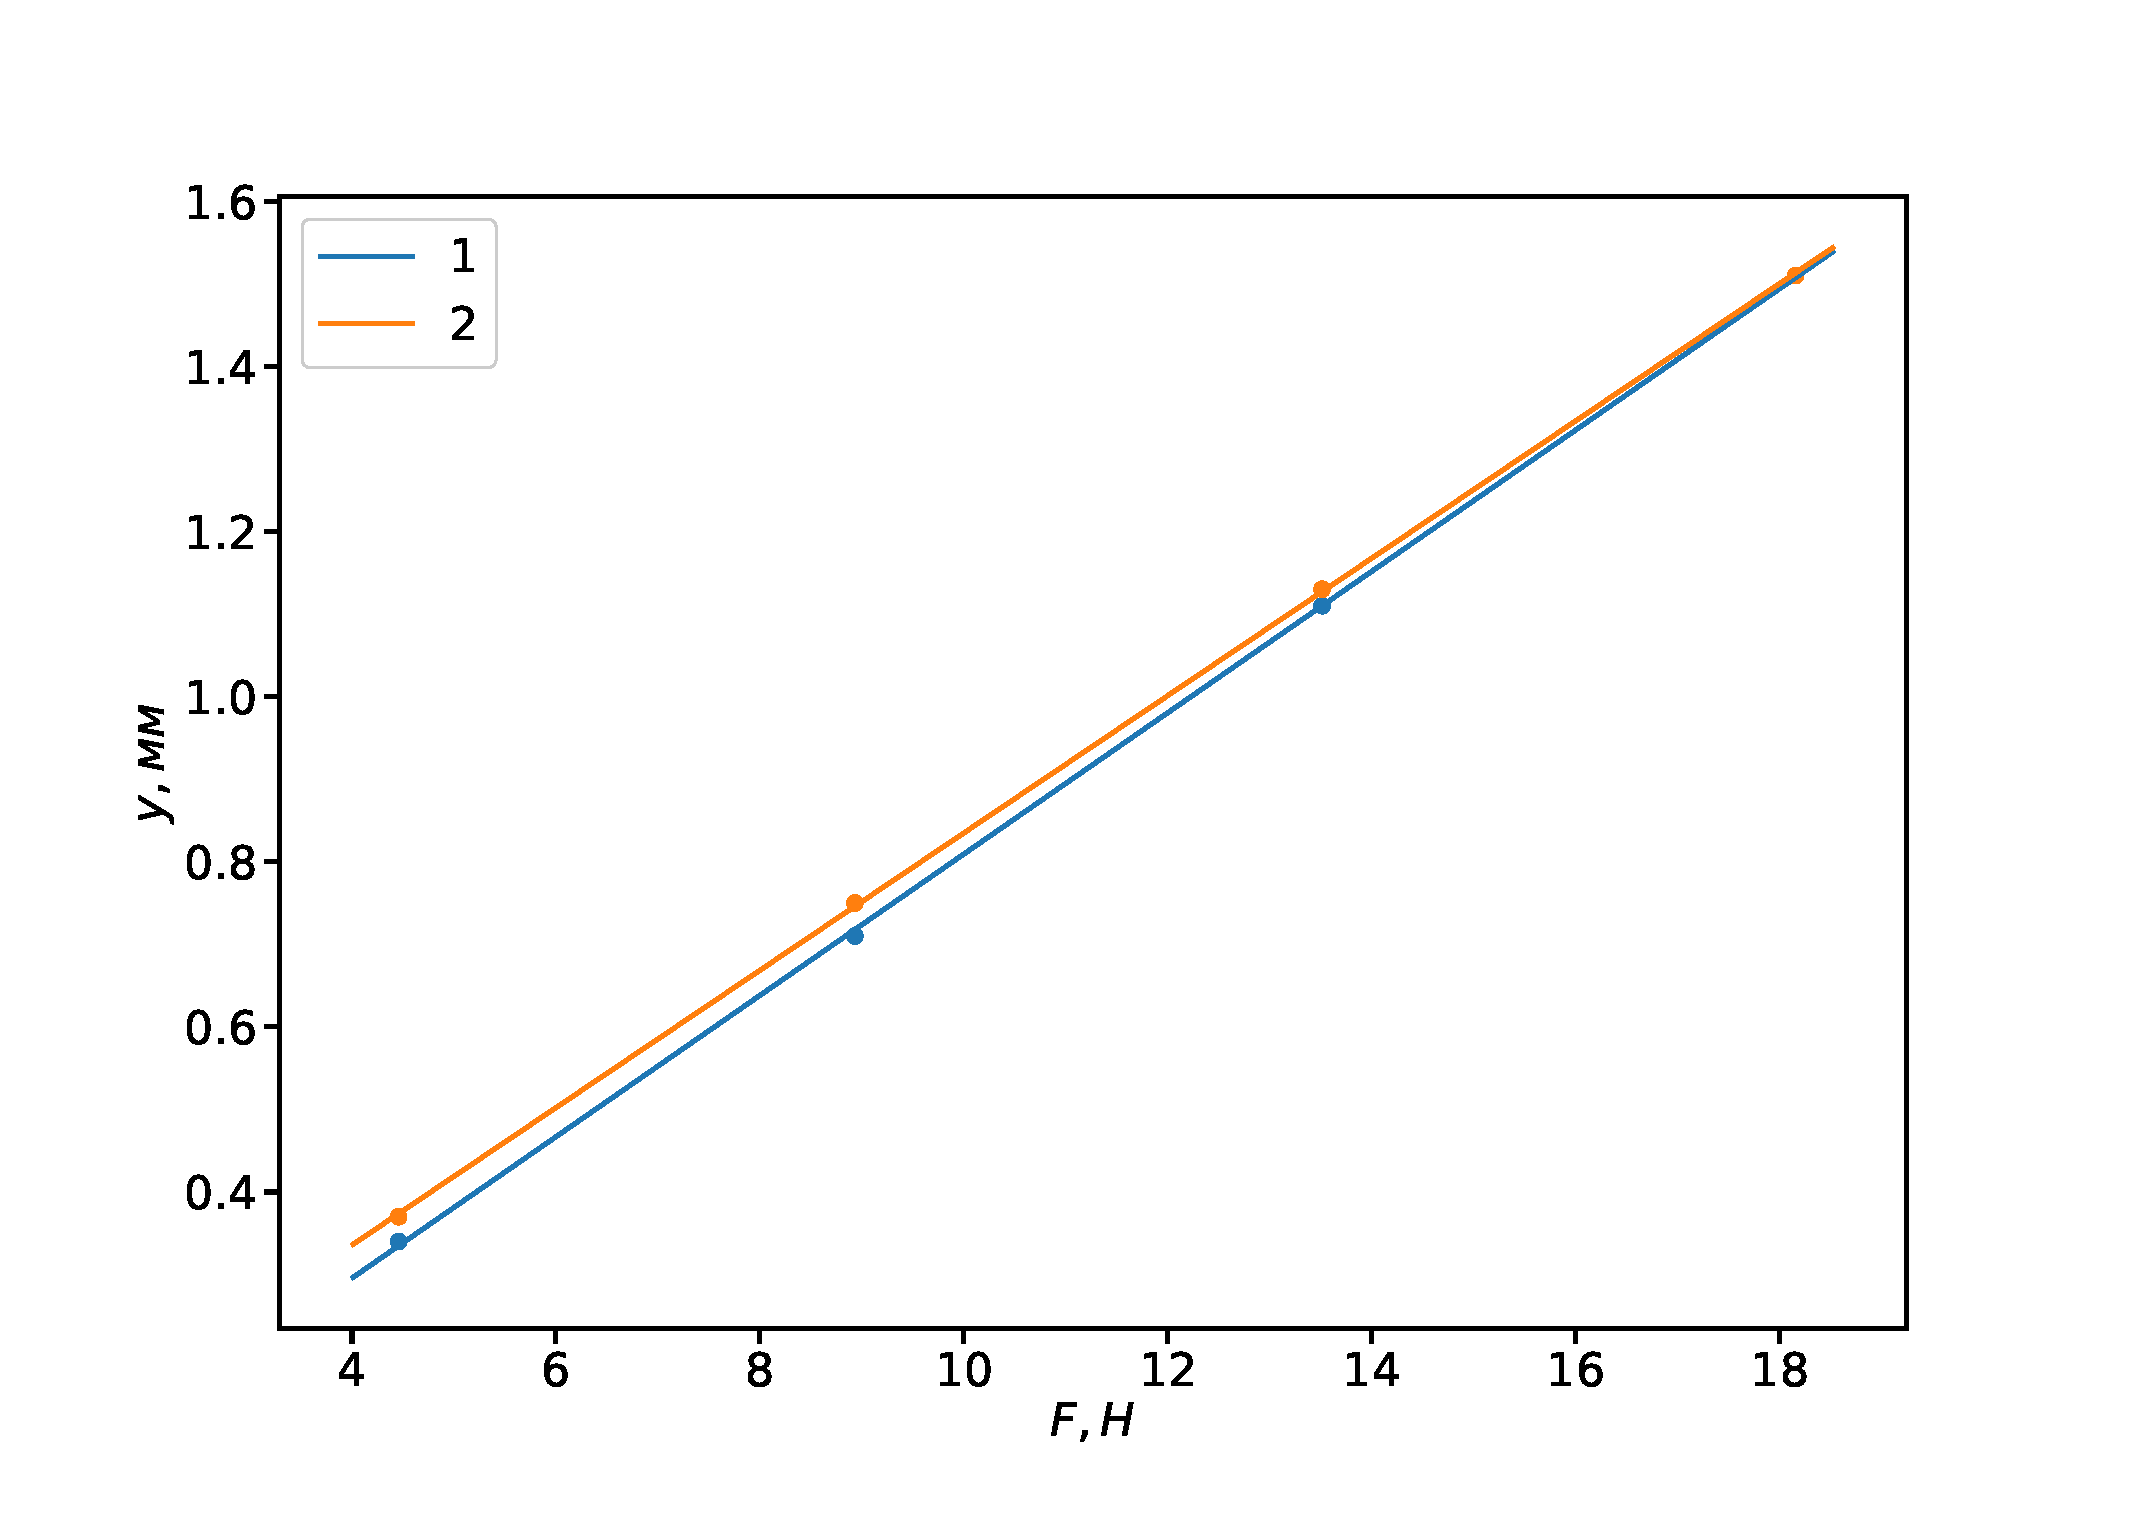
\includegraphics[width=0.6\textwidth]{groupdown_wood1.eps}
    \end{center}
    \caption{Графики зависимости максимального прогиба дубовой балки $y$ от приложенной нагрузки $F$. 1 - измерение на увеличение нагрузки.
        2 - измерение на уменьшение нагрузки.}
    \label{fig:3}
\end{figure}

\begin{figure}[H]
    \begin{center}
        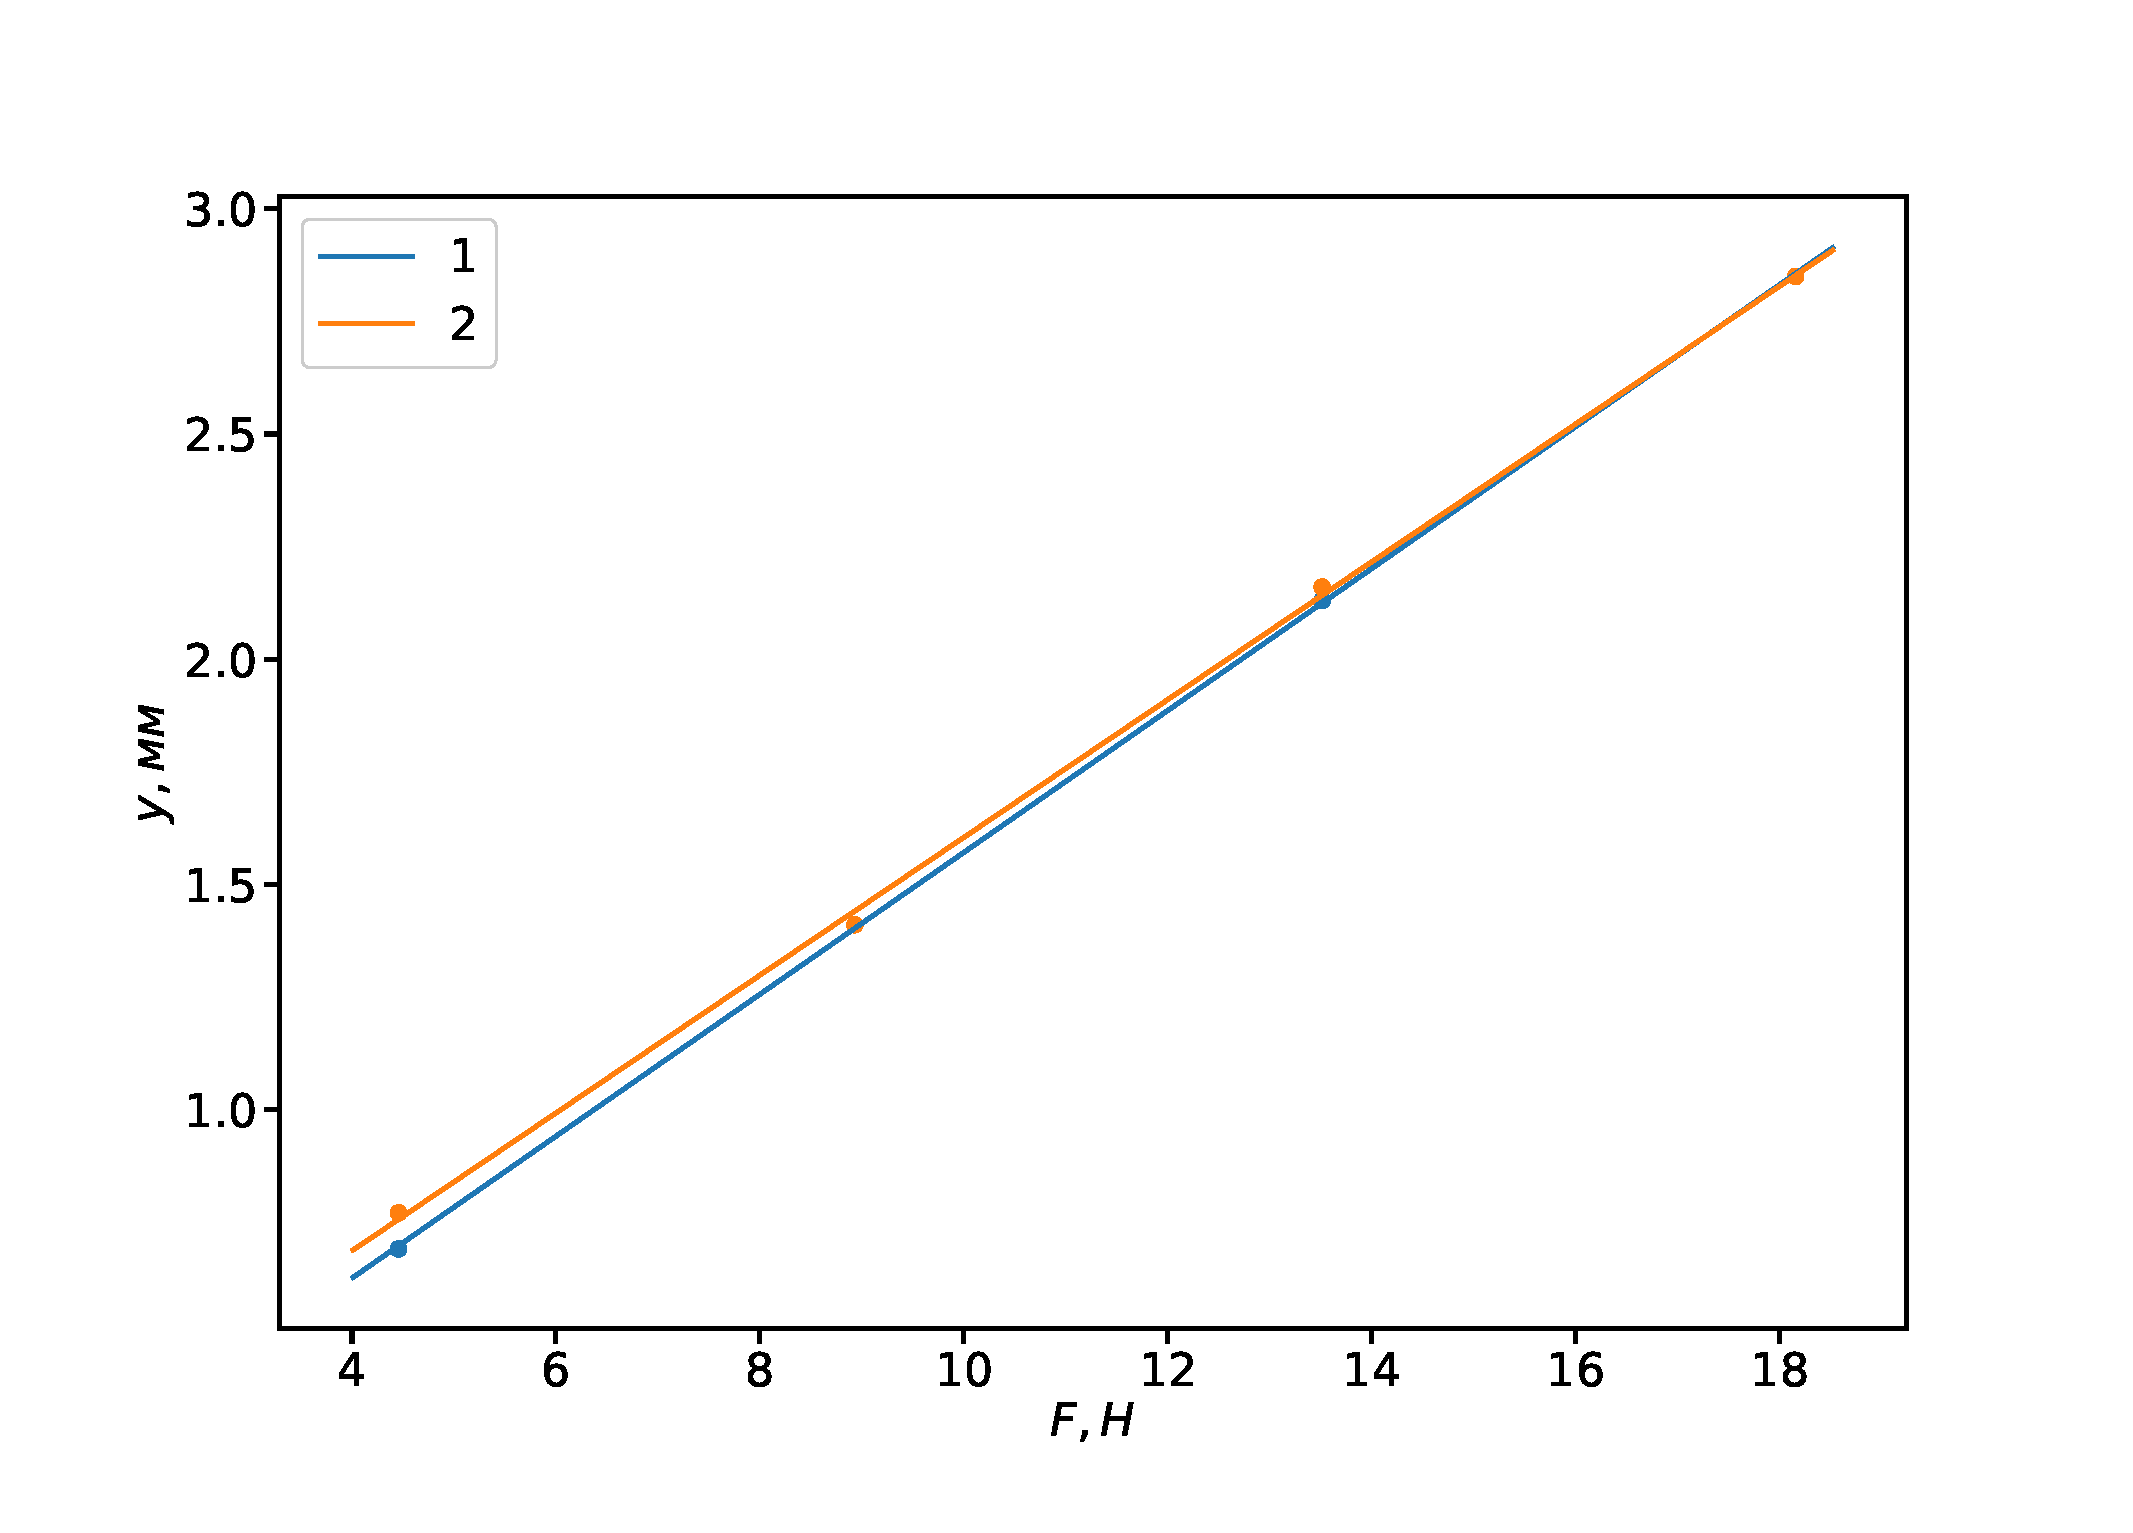
\includegraphics[width=0.6\textwidth]{groupdown_wood2.eps}
    \end{center}
    \caption{Графики зависимости максимального прогиба еловой балки $y$ от приложенной нагрузки $F$. 1 - измерение на увеличение нагрузки.
        2 - измерение на уменьшение нагрузки.}
    \label{fig:4}
\end{figure}

Для железной балки коэффициент наклона не зависит от направления измерения. Для деревянных балок присутствует небольшая зависимость коэффициента
наклона от направления измерения.

\begin{figure}[H]
    \begin{center}
        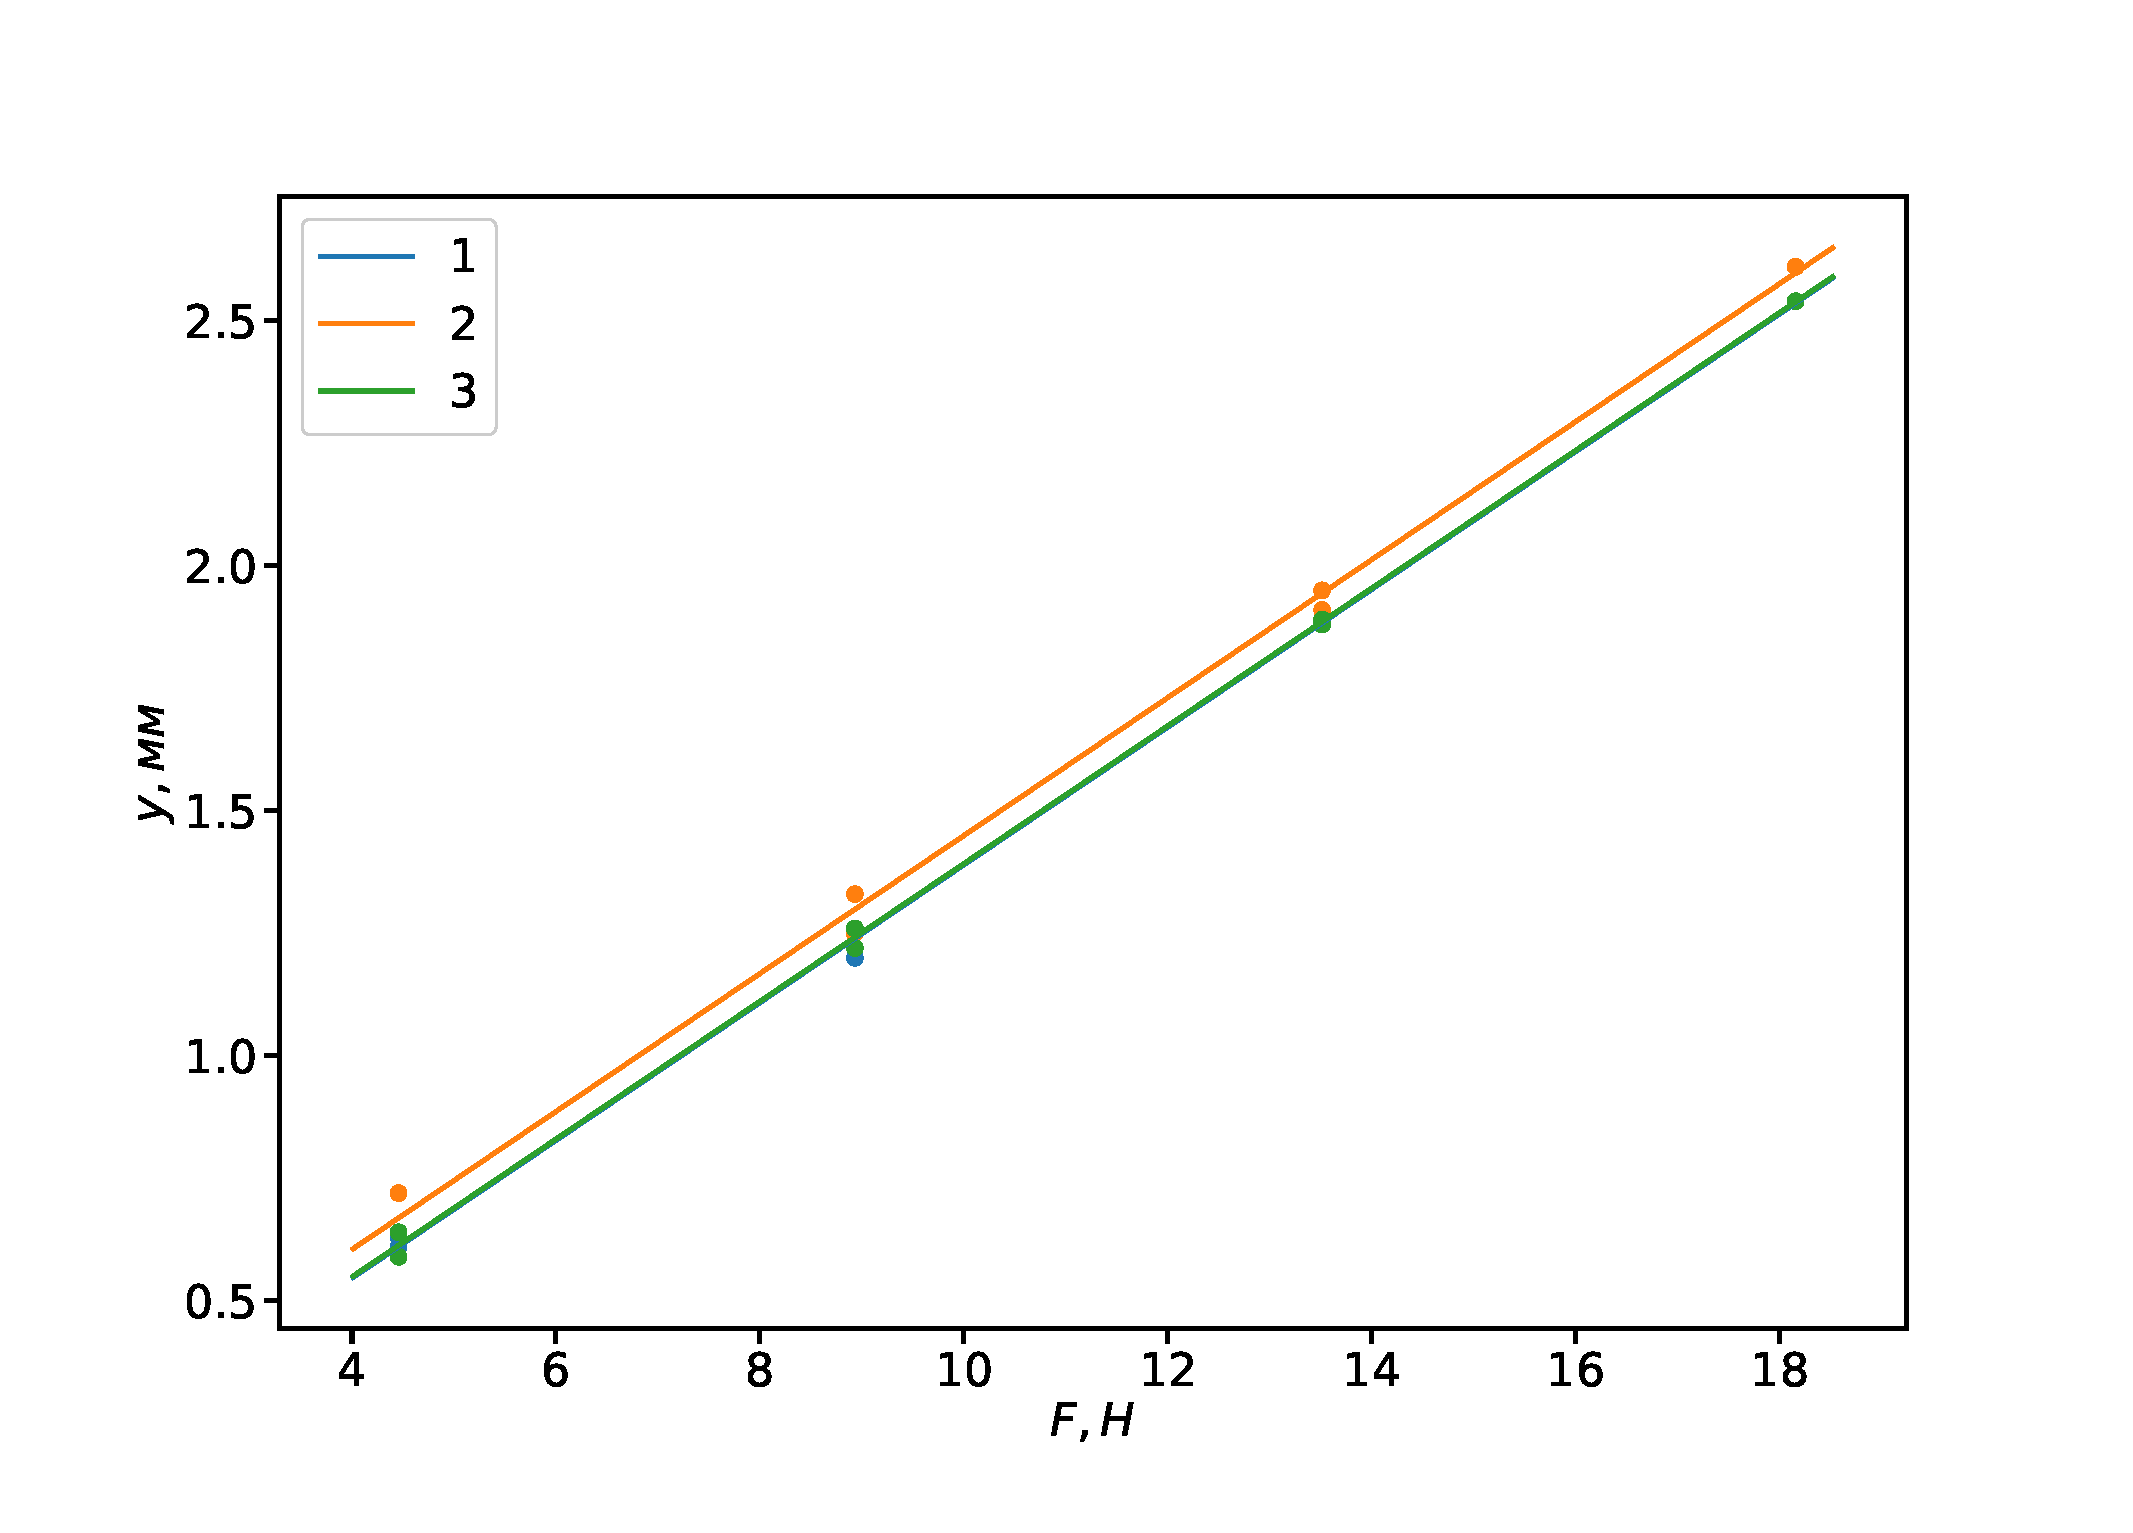
\includegraphics[width=0.6\textwidth]{gr1.eps}
    \end{center}
    \caption{Графики зависимости максимального прогиба железной балки $y$ от приложенной нагрузки $F$. 1 - прямое измерение прогиба,
        2 - измерение прогиба перевёрнутой балки, 3 - измерение прогиба балки со смещённой точкой приложения нагрузки}
    \label{fig:5}
\end{figure}

\begin{figure}[H]
    \begin{center}
        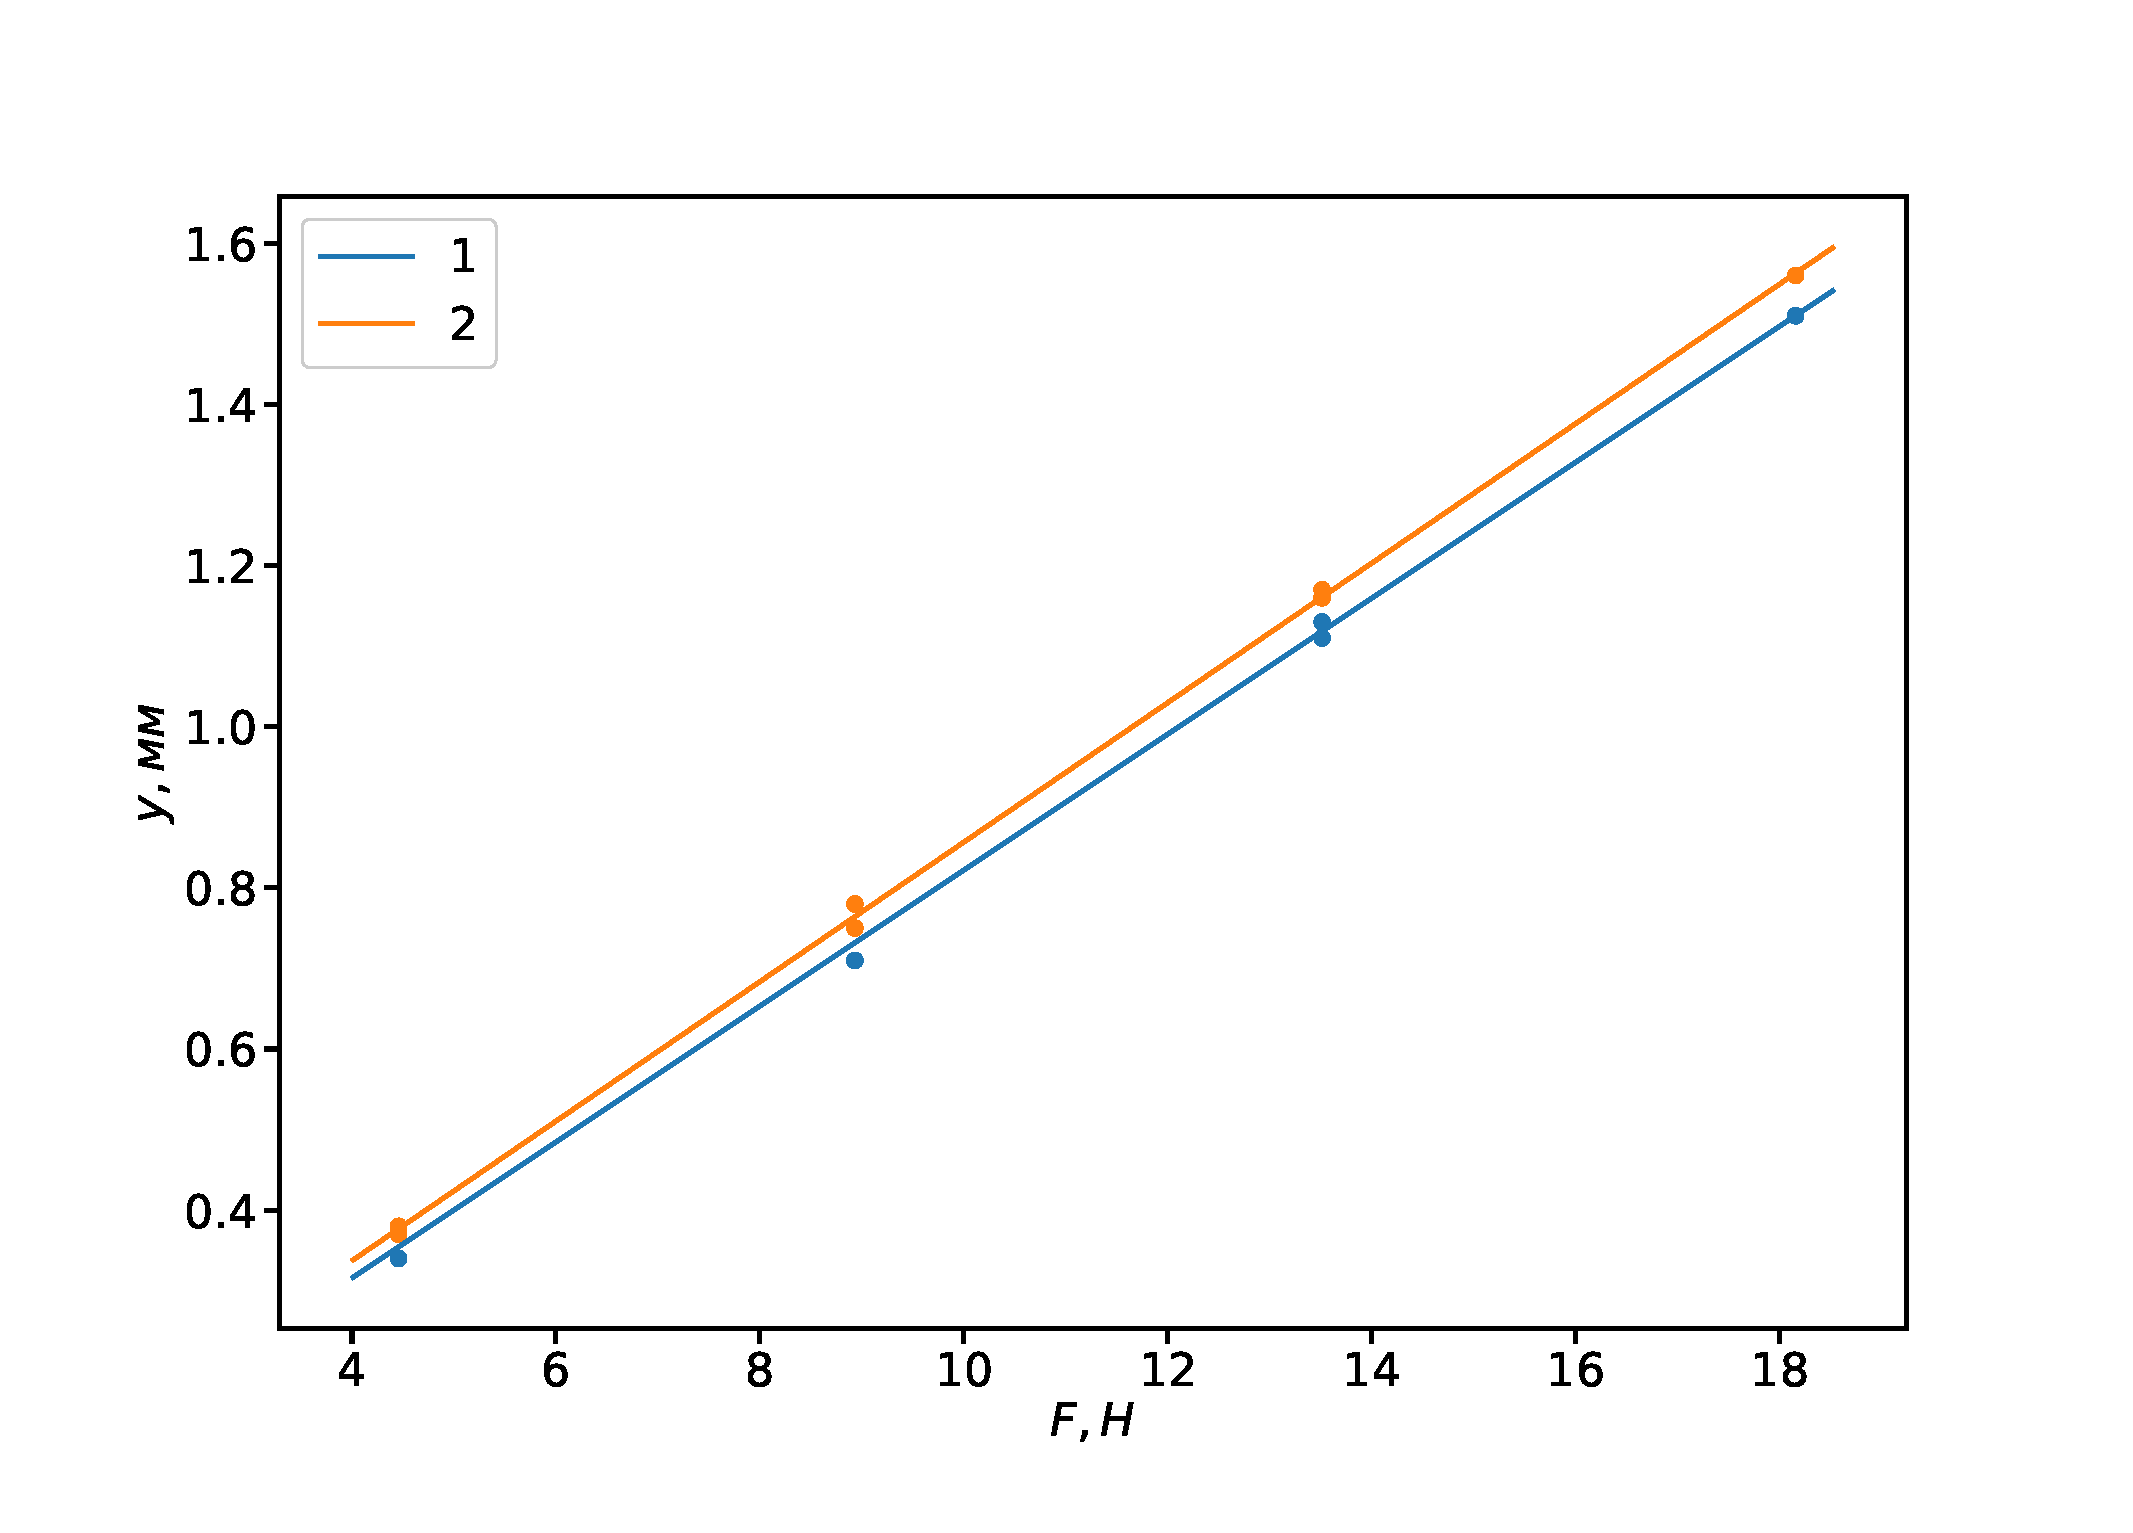
\includegraphics[width=0.6\textwidth]{gr2.eps}
    \end{center}
    \caption{Графики зависимости максимального прогиба дубовой балки $y$ от приложенной нагрузки $F$. 1 - прямое измерение прогиба,
        2 - измерение прогиба перевёрнутой балки}
    \label{fig:6}
\end{figure}

\begin{figure}[H]
    \begin{center}
        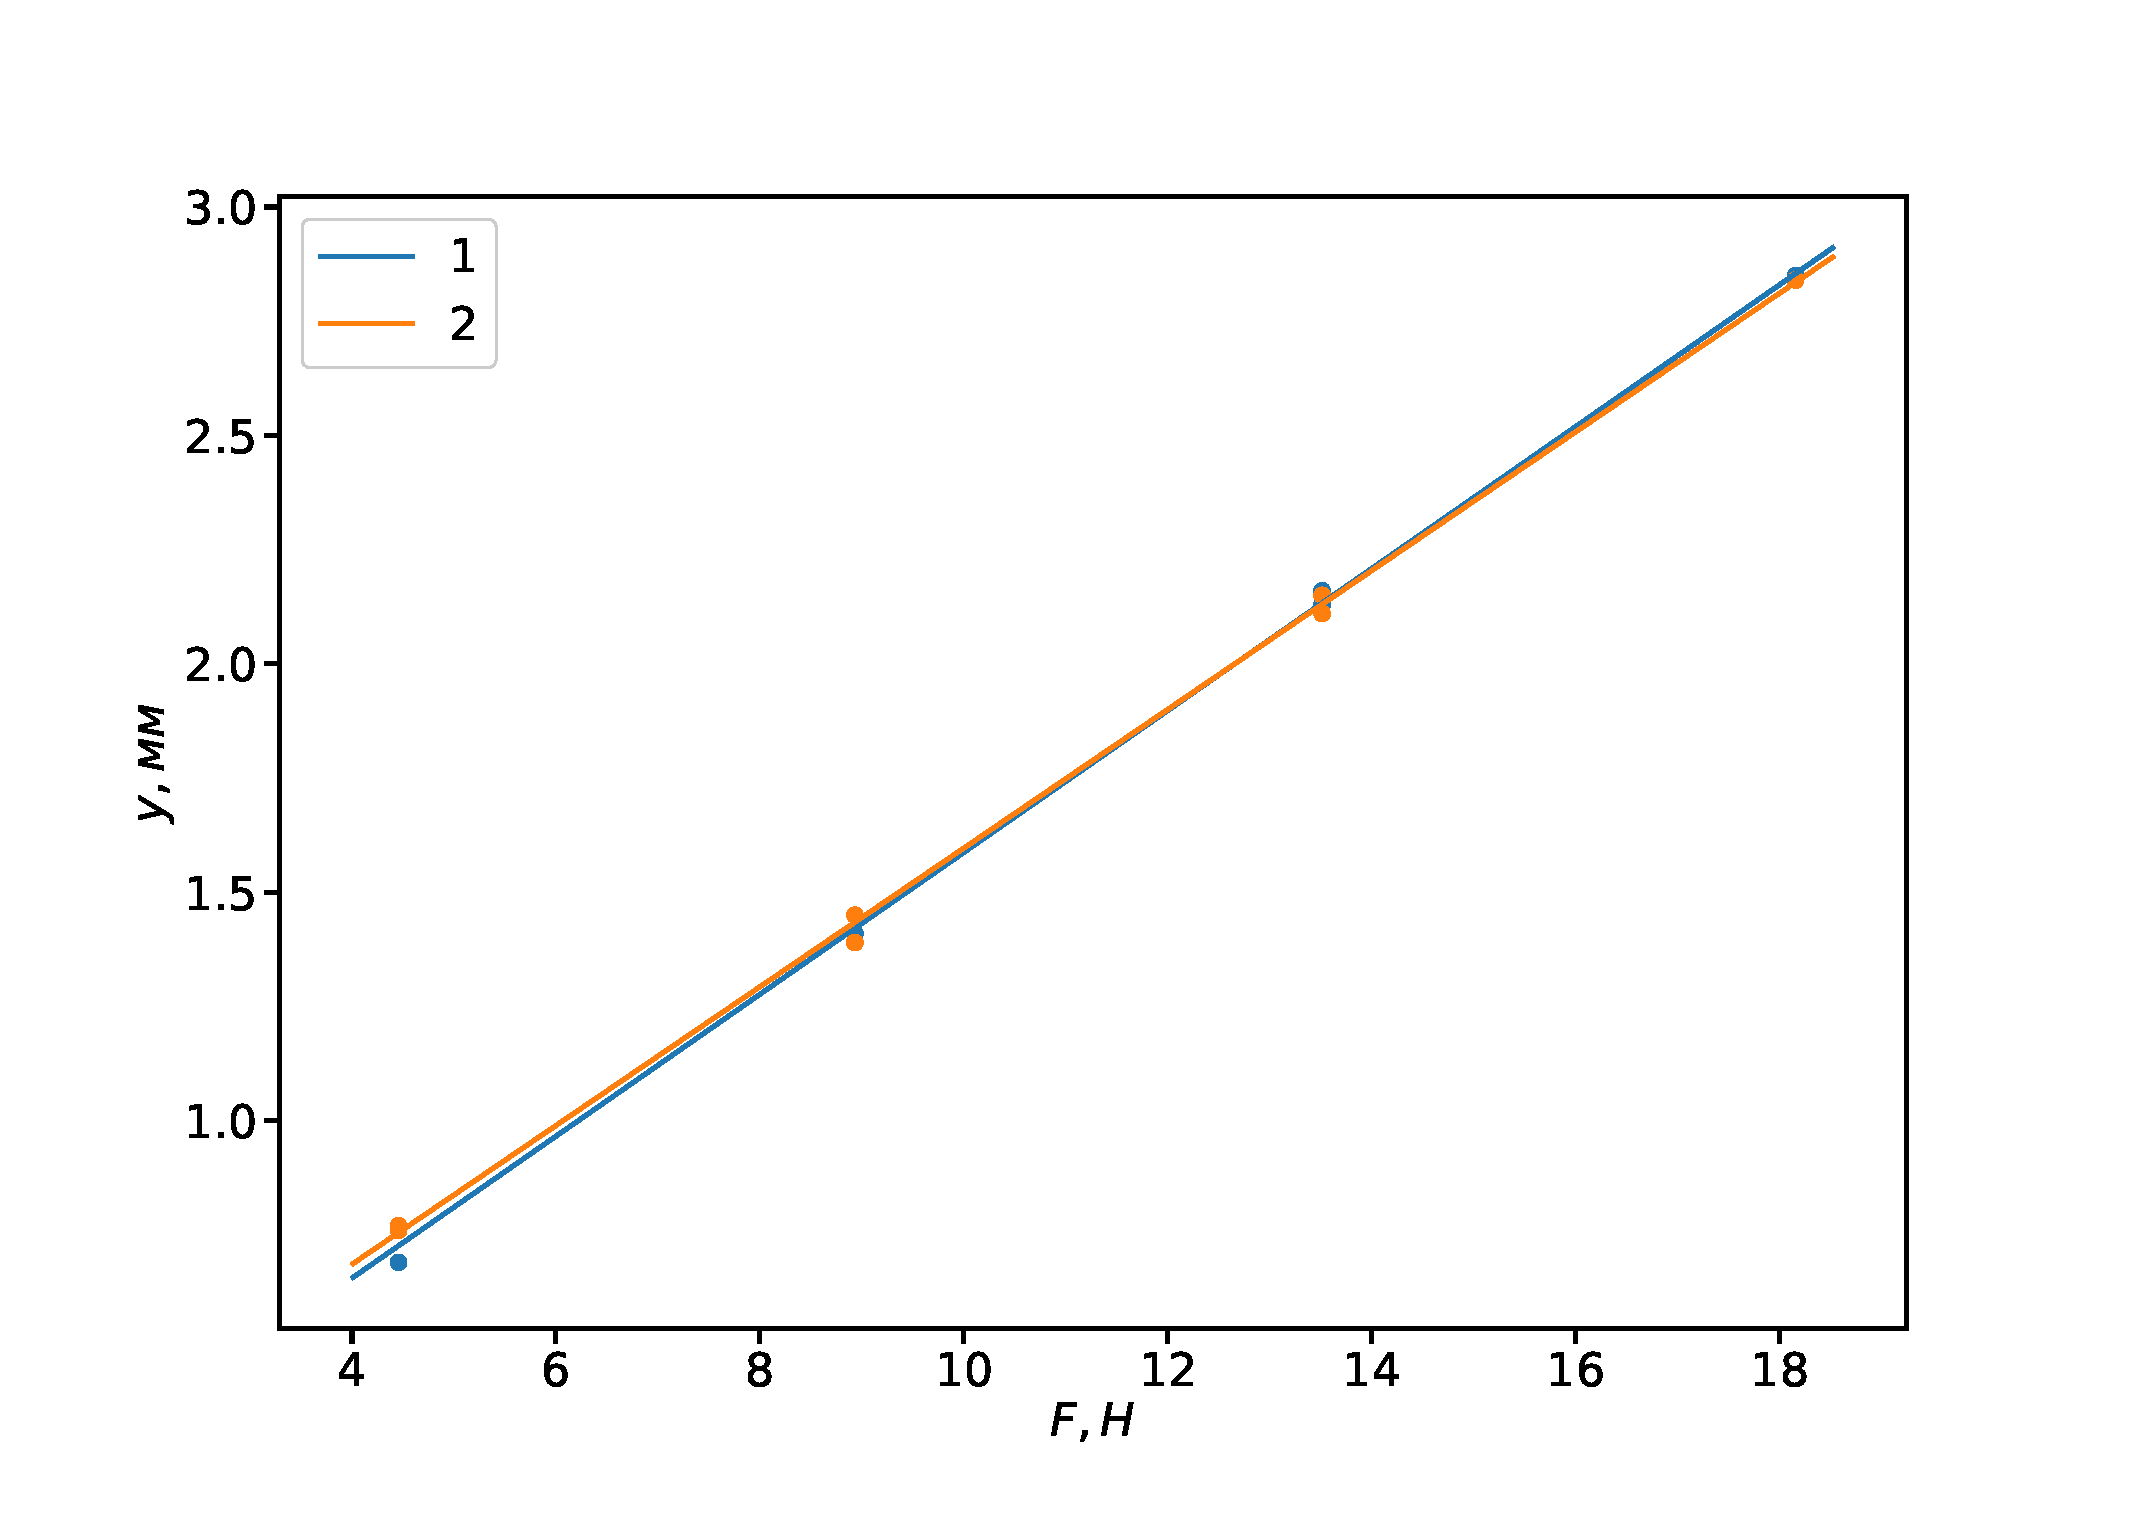
\includegraphics[width=0.6\textwidth]{gr3.eps}
    \end{center}
    \caption{Графики зависимости максимального прогиба еловой балки $y$ от приложенной нагрузки $F$. 1 - прямое измерение прогиба,
        2 - измерение прогиба перевёрнутой балки}
    \label{fig:7}
\end{figure}

Согласно графику \ref{fig:5} для железной балки зависимость со смещённой точкой приложения механического механического напряжения неразличима с прямой зависимостью, также у 
железной балки наблюдается смещение графика зависимости для перевёрнутого случая из-за пластической деформации. Для деревянных балок 
зависимость для перевёрнутой и неперевёрнутой балки почти не отличаются. 

\subsection{Метод наименьших квадратов} \label{app_4}
$$y = a + bx$$
Формула для расчёта коэффициентов $a$ и $b$:
$$b = \frac{\overline{xy} - \overline{x}\overline{y}}{\overline{x^2} - \overline{x}^2}$$
$$a = \overline{y} - b\overline{x}$$
Погрешности:
$$\sigma_b \approx \frac{1}{\sqrt{n}}\sqrt{\frac{\overline{y^2} - \overline{y}^2}{\overline{x^2} - \overline{x}^2} - b^2}$$
$$\sigma_a \approx \sigma_b \sqrt{\overline{x^2} - \overline{x}^2}$$
\end{document}